% !TEX encoding = UTF-8 Unicode
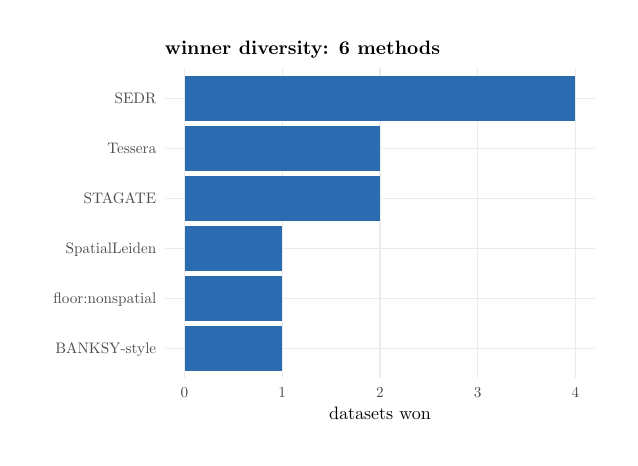
\begin{tikzpicture}[x=1pt,y=1pt]
\definecolor{fillColor}{RGB}{255,255,255}
\path[use as bounding box,fill=fillColor,fill opacity=0.00] (0,0) rectangle (210.44,148.14);
\begin{scope}
\path[clip] (  1.45,  1.84) rectangle (209.00,146.30);
\definecolor{fillColor}{RGB}{255,255,255}

\path[fill=fillColor] (  1.45,  1.84) rectangle (209.00,146.30);
\end{scope}
\begin{scope}
\path[clip] ( 49.61, 21.41) rectangle (205.00,133.43);
\definecolor{drawColor}{gray}{0.92}

\path[draw=drawColor,line width= 0.4pt,line join=round] ( 49.61, 32.25) --
	(205.00, 32.25);

\path[draw=drawColor,line width= 0.4pt,line join=round] ( 49.61, 50.32) --
	(205.00, 50.32);

\path[draw=drawColor,line width= 0.4pt,line join=round] ( 49.61, 68.38) --
	(205.00, 68.38);

\path[draw=drawColor,line width= 0.4pt,line join=round] ( 49.61, 86.45) --
	(205.00, 86.45);

\path[draw=drawColor,line width= 0.4pt,line join=round] ( 49.61,104.52) --
	(205.00,104.52);

\path[draw=drawColor,line width= 0.4pt,line join=round] ( 49.61,122.59) --
	(205.00,122.59);

\path[draw=drawColor,line width= 0.4pt,line join=round] ( 56.68, 21.41) --
	( 56.68,133.43);

\path[draw=drawColor,line width= 0.4pt,line join=round] ( 91.99, 21.41) --
	( 91.99,133.43);

\path[draw=drawColor,line width= 0.4pt,line join=round] (127.30, 21.41) --
	(127.30,133.43);

\path[draw=drawColor,line width= 0.4pt,line join=round] (162.62, 21.41) --
	(162.62,133.43);

\path[draw=drawColor,line width= 0.4pt,line join=round] (197.93, 21.41) --
	(197.93,133.43);
\definecolor{fillColor}{RGB}{43,108,176}

\path[fill=fillColor] ( 56.68, 24.12) rectangle ( 91.99, 40.38);

\path[fill=fillColor] ( 56.68, 42.19) rectangle ( 91.99, 58.45);

\path[fill=fillColor] ( 56.68,114.46) rectangle (197.93,130.72);

\path[fill=fillColor] ( 56.68, 60.25) rectangle ( 91.99, 76.51);

\path[fill=fillColor] ( 56.68, 78.32) rectangle (127.30, 94.58);

\path[fill=fillColor] ( 56.68, 96.39) rectangle (127.30,112.65);
\end{scope}
\begin{scope}
\path[clip] (  0.00,  0.00) rectangle (210.44,148.14);
\definecolor{drawColor}{gray}{0.30}

\node[text=drawColor,anchor=base east,inner sep=0pt, outer sep=0pt, scale=  0.55] at ( 46.46, 30.35) {BANKSY-style};

\node[text=drawColor,anchor=base east,inner sep=0pt, outer sep=0pt, scale=  0.55] at ( 46.46, 48.42) {floor:nonspatial};

\node[text=drawColor,anchor=base east,inner sep=0pt, outer sep=0pt, scale=  0.55] at ( 46.46, 66.49) {SpatialLeiden};

\node[text=drawColor,anchor=base east,inner sep=0pt, outer sep=0pt, scale=  0.55] at ( 46.46, 84.56) {STAGATE};

\node[text=drawColor,anchor=base east,inner sep=0pt, outer sep=0pt, scale=  0.55] at ( 46.46,102.62) {Tessera};

\node[text=drawColor,anchor=base east,inner sep=0pt, outer sep=0pt, scale=  0.55] at ( 46.46,120.69) {SEDR};
\end{scope}
\begin{scope}
\path[clip] (  0.00,  0.00) rectangle (210.44,148.14);
\definecolor{drawColor}{gray}{0.30}

\node[text=drawColor,anchor=base,inner sep=0pt, outer sep=0pt, scale=  0.55] at ( 56.68, 14.47) {0};

\node[text=drawColor,anchor=base,inner sep=0pt, outer sep=0pt, scale=  0.55] at ( 91.99, 14.47) {1};

\node[text=drawColor,anchor=base,inner sep=0pt, outer sep=0pt, scale=  0.55] at (127.30, 14.47) {2};

\node[text=drawColor,anchor=base,inner sep=0pt, outer sep=0pt, scale=  0.55] at (162.62, 14.47) {3};

\node[text=drawColor,anchor=base,inner sep=0pt, outer sep=0pt, scale=  0.55] at (197.93, 14.47) {4};
\end{scope}
\begin{scope}
\path[clip] (  0.00,  0.00) rectangle (210.44,148.14);
\definecolor{drawColor}{RGB}{0,0,0}

\node[text=drawColor,anchor=base,inner sep=0pt, outer sep=0pt, scale=  0.65] at (127.30,  6.38) {datasets won};
\end{scope}
\begin{scope}
\path[clip] (  0.00,  0.00) rectangle (210.44,148.14);
\definecolor{drawColor}{RGB}{0,0,0}

\node[text=drawColor,anchor=base west,inner sep=0pt, outer sep=0pt, scale=  0.70] at ( 49.61,138.47) {\bfseries winner diversity: 6 methods};
\end{scope}
\end{tikzpicture}
